\documentclass[11pt,a4paper]{article}
\usepackage[margin=26mm,headheight=14pt]{geometry}
\usepackage{fontspec}
\setmainfont{Latin Modern Roman}[Ligatures=TeX]
\setsansfont{Latin Modern Sans}[Scale=0.95]
\setmonofont{Latin Modern Mono}[Scale=0.9]
\usepackage{amsmath,amsthm,amssymb,mathtools}
\usepackage{microtype,booktabs,longtable,array,enumitem,graphicx,xcolor}
\usepackage{tikz}
\usetikzlibrary{arrows.meta,positioning,calc}
\usepackage{fancyhdr,needspace}
\definecolor{ink}{HTML}{173D49}
\definecolor{teal}{HTML}{176F76}
\definecolor{muted}{HTML}{58616B}
\usepackage[unicode,colorlinks=true,linkcolor=ink,citecolor=teal,urlcolor=teal,
 pdftitle={Uniform avoidance of geometric progressions and exponential-polynomial patterns},
 pdfauthor={Research manuscript prepared with ChatGPT for Vladimir Reshetnikov}]{hyperref}
\usepackage[nameinlink,noabbrev]{cleveref}
\usepackage{titlesec}
\titleformat{\section}{\Large\bfseries\color{ink}}{\thesection}{0.7em}{}
\titleformat{\subsection}{\large\bfseries\color{ink}}{\thesubsection}{0.7em}{}
\setlength{\parskip}{3pt}
\setlength{\emergencystretch}{2em}
\setlist{itemsep=2pt,topsep=5pt}
\pagestyle{fancy}\fancyhf{}
\fancyhead[L]{\small\color{muted}Uniform geometric avoidance}
\fancyhead[R]{\small\color{muted}7 October 2026}
\fancyfoot[C]{\thepage}
\renewcommand{\headrulewidth}{0.3pt}
\theoremstyle{plain}
\newtheorem{theorem}{Theorem}[section]
\newtheorem{proposition}[theorem]{Proposition}
\newtheorem{lemma}[theorem]{Lemma}
\newtheorem{corollary}[theorem]{Corollary}
\theoremstyle{definition}
\newtheorem{definition}[theorem]{Definition}
\newtheorem{question}{Research question}
\theoremstyle{remark}
\newtheorem{remark}[theorem]{Remark}
\newcommand{\R}{\mathbb R}\newcommand{\N}{\mathbb N}\newcommand{\Z}{\mathbb Z}
\newcommand{\Q}{\mathbb Q}\newcommand{\E}{\mathbb E}
\newcommand{\Prob}{\mathbb P}\newcommand{\ind}{\mathbf 1}
\newcommand{\calS}{\mathcal S}\newcommand{\calA}{\mathcal A}
\newcommand{\calF}{\mathcal F}\newcommand{\calI}{\mathcal I}
\newcommand{\dist}{\operatorname{dist}}\newcommand{\sgn}{\operatorname{sgn}}
\newcommand{\GP}{G_q}\newcommand{\eps}{\varepsilon}
\DeclareMathOperator{\supp}{supp}
\begin{document}
\hypersetup{pageanchor=false}
\begin{titlepage}
\raggedright
\vspace*{12mm}
{\sffamily\small\color{teal}RESEARCH ARTICLE \quad / \quad ANALYSIS, COMBINATORICS, COMPUTABILITY}\par
\vspace{12mm}
{\Huge\bfseries\color{ink}Uniform avoidance of geometric progressions\par}
\vspace{5mm}
{\LARGE\color{ink}and exponential-polynomial patterns\par}
\vspace{9mm}
{\large Common periodic avoiding sets\par
and effective finite certificates}\par
\vspace{13mm}
{\large Prepared for Vladimir Reshetnikov}\par
{\color{muted}Mathematical development and exposition with ChatGPT}\par
{\color{muted}7 October 2026}\par
\vspace{10mm}
\begin{abstract}
We prove that, for every $\eps>0$, there is a closed, symmetric, $1$-periodic set
$F\subset\R$ whose measure in every interval of length one exceeds $1-\eps$
and which contains no affine copy of $\{q^n:n\ge1\}$ for \emph{any}
$q\in(0,1)$. Its compact section answers negatively Question~1 of
Burgin--Goldberg--Keleti--MacMahon--Wang. The construction extends the
fixed-ratio routing method in the October 2026 OpenAI manuscript by
synchronizing a ratio-dependent subsequence to common spatial grids.
An elementary arrangement of lines bounds the number of parameter tests,
including boundary cases. A polynomial-family version, using the classical
bound for realizable polynomial sign conditions, yields one common avoiding
set for every finite positive exponential mixture
$\sum_{i=1}^m c_iq_i^n$, with unrestricted finite $m$, positive bases below
one, and nonnegative coefficients not all zero. A uniform dominant-term
reduction also covers arbitrary real polynomial coefficients with positive
real bases, and hence all nonzero real solutions of homogeneous
constant-coefficient recurrences whose characteristic roots lie in $(0,1)$.
For rational accuracy the
compact set can be effectively closed with computable Lebesgue measure.
Finite avoidance statements on rational compact parameter boxes have
algorithmically obtainable rational certificates and positive margins.
The probability argument is given in full; exact finite checks accompany
the article. The similarity conjecture for arbitrary infinite patterns remains
outside the conclusions of this paper.
\end{abstract}
\vfill
{\small\color{muted}Research status. Complete proofs are presented here, with explicit attribution
of the inherited construction and the new extensions. This manuscript has
not undergone external peer review or Lean formalization. The accompanying
computations check finite identities and invariants; they are not a substitute
for the proofs.}
\end{titlepage}
\hypersetup{pageanchor=true}
\begingroup
\small
\setlength{\parskip}{0pt}
\tableofcontents
\endgroup
\clearpage
\section{The question, the results, and their provenance}
\label{sec:context}

Throughout the paper $m$ is Lebesgue measure and $\N=\{1,2,\ldots\}$.
For a measurable $1$-periodic set $H$ write
\[
 \rho(H)=m(H\cap[0,1)).
\]
A nontrivial affine copy of a set $A\subset\R$ has the form $x+sA$,
where $x\in\R$ and $s\ne0$. Put $G_q=\{q^n:n\ge1\}$ for $0<q<1$.
The distinction between one fixed $q$ and the entire continuum of ratios
is central to the results.

\subsection{A published question with different quantifiers}

The Erd\H{o}s similarity conjecture asks whether every infinite subset of
$\R$ has a positive-measure set avoiding all its nontrivial affine copies.
Burgin, Goldberg, Keleti, MacMahon, and Wang posed the following separate
question in \cite[Question~1]{BGKMW}: must every measurable set of positive
measure contain $\{x+sq^n:n\ge1\}$ for \emph{some} triple $(x,s,q)$ with
$s\ne0$ and $0<q<1$? A negative answer requires a single set that excludes
all three parameters at once.

Theorem~1.1 of their paper constructs a compact set having zero as a density
point but containing no unshifted progression $\{sq^n:n\ge1\}$. That result
does not exclude progressions converging to another center. Their
almost-everywhere avoidance statement also leaves exceptional parameter
values. The survey \cite{JLM} provides the historical context; it predates
the October 2026 manuscript used below.

The OpenAI manuscript \cite[Theorem~1.1]{OpenAI84} proves that for each
\emph{fixed} $q$ there are compact subsets of $[0,1]$ of measure arbitrarily
close to one avoiding all affine copies of $G_q$. Its introduction explicitly
permits the avoiding set to depend on $q$. Summable intersections therefore
handle any specified countable collection of ratios. They do not by
themselves handle every real ratio. This paper supplies that missing
uniform argument.

\begin{theorem}[Uniform geometric avoidance]\label{thm:main}
For every $0<\eps<1$ there exists a closed, symmetric, $1$-periodic set
$F_\eps\subset\R$ such that
\begin{equation}\label{eq:main-density}
 m(F_\eps\cap[u,u+1])\ge1-\frac\eps2>1-\eps
 \qquad(u\in\R),
\end{equation}
and, for every $x\in\R$, $s\in\R\setminus\{0\}$, and $q\in(0,1)$,
\begin{equation}\label{eq:main-avoidance}
 x+sq^n\notin F_\eps\quad\text{for infinitely many }n\ge1.
\end{equation}
Consequently $K_\eps=F_\eps\cap[0,1]$ is compact, has measure greater
than $1-\eps$, and answers \cite[Question~1]{BGKMW} negatively.
\end{theorem}

The conclusion is stronger than avoidance at a prescribed limit point.
Every point, every signed dilation, and every contracting ratio are covered
by the same set. Periodicity in \cref{thm:main} is possible because passing
to a tail of a geometric progression reduces its scale. The construction
only needs dyadic contractions of periodic sets.

\begin{theorem}[All finite positive exponential mixtures]\label{thm:mixtures}
For every $0<\eps<1$ there is a closed, symmetric, $1$-periodic set
$F^*_\eps\subset\R$ satisfying \eqref{eq:main-density} and the following
property. For every finite $d\ge1$, every $q_1,\ldots,q_d\in(0,1)$,
every $c_1,\ldots,c_d\ge0$ with $\sum_i c_i>0$, every $x\in\R$, and
every $s\ne0$, infinitely many terms of
\begin{equation}\label{eq:mixture-orbit}
 x+s\sum_{i=1}^d c_iq_i^n,\qquad n\ge1,
\end{equation}
lie outside $F^*_\eps$. All choices, including the number $d$ of
components, are simultaneous.
\end{theorem}

The terms in \eqref{eq:mixture-orbit} are synchronized sums: the exponent
$n$ is the same in every summand. This is a different pattern from the
sumset in which all component exponents vary independently. Repeated
bases and zero coefficients are allowed. The proof is an application of
a general theorem for finite-dimensional polynomial families in
\cref{sec:algebraic}. That section also proves a stronger extension to
all nonzero real exponential polynomials with positive real bases,
allowing signed coefficients, and deduces the corresponding theorem
for homogeneous constant-coefficient real recurrences with roots in $(0,1)$.

\begin{theorem}[Effective compact sets and finite margins]\label{thm:effective-intro}
For rational $0<\eps<1$, the compact sets in \cref{thm:main,thm:mixtures}
can be chosen effectively closed, uniformly in $\eps$, with computable
Lebesgue measure. More precisely, they have nested approximations $K_N$
by finite unions of closed rational intervals such that
\begin{equation}\label{eq:effective-rate-intro}
 K=\bigcap_{N\ge1}K_N,
 \qquad 0\le m(K_N)-m(K)\le\eps\,2^{-N}.
\end{equation}
For any rational compact parameter box contained in the admissible domain,
with the dilation bounded away from zero, one can algorithmically obtain a finite index bound and a
positive rational avoidance margin. The precise certificate is given in
\cref{thm:certificates}.
\end{theorem}

Effectively closed here means that the open complement can be enumerated
as a union of rational open intervals. It does not assert decidable
membership, or computability in the Hausdorff representation of compact
sets. The finite search procedures proved to terminate below are not
claimed to be efficient.

\subsection{What was reviewed and what is new}

The repository review used the revisions recorded in \cref{sec:provenance}.
The OpenAI catalogue contains manuscripts at different verification stages;
its own README makes that distinction \cite{OpenAICatalog}. We inspected
the actual source of the geometric similarity manuscript, not just its
catalogue description. In ProveIt we reviewed the repository overview,
Ramsey refinement status, and selected matching and analysis material
\cite{ProveIt}. The large collection of existing Gowers refinements made
another minor local refinement a less attractive target. The present
question offers a precise published target and a useful connection to
ProveIt's work on exact certificates, polynomial decision procedures, and
exponential sequences.

\begin{center}
\begin{tabular}{@{}>{\raggedright\arraybackslash}p{0.30\textwidth}>{\raggedright\arraybackslash}p{0.62\textwidth}@{}}
\toprule
Ingredient & Status in this article\\
\midrule
Ordered-tree routing; selector and terminal tables & Adapted, with full
attribution, from the fixed-ratio proof in \cite{OpenAI84}. The probability
argument is reproduced in our notation and checked directly.\\[3pt]
Common-scale subsequence for varying $q$ & New uniformization step:
$\nu_j(q)=\min\{n:q^n\le Q^j\}$. The random set is independent of $q$.\\[3pt]
Two-parameter cell count & New use of lines in logarithmic coordinates,
including jump points, edges, and vertices.\\[3pt]
Polynomial-family extension & New application of the classical
sign-condition bound \cite{BPR}; yields \cref{thm:mixtures}.\\[3pt]
Periodic global assembly and effective certificates & Developed here;
uses tail closure, summable budgets, and real quantifier elimination.\\
\bottomrule
\end{tabular}
\end{center}

The principal theorem is proved with finite probability and elementary
measure theory. The general polynomial-family extension additionally uses
a stated classical theorem of real algebraic geometry. The effective
results use decidability of real polynomial inequalities. No flagship
claim elsewhere in either repository is an unproved hypothesis of these
arguments.

\subsection{Road map}

We first synchronize all ratios in a compact interval to one family of
spatial scales. A finite tree gives independent opportunities for a hit
while keeping the mean measure small. The first default choice in the
route of a fixed center identifies the relevant tests. A line arrangement
then replaces the continuum of ratio--dilation parameters by finitely many
representatives. Compactness repairs the remaining centers. Finally,
countable summable assembly covers all ratios and scales. The same scheme
with polynomial sign conditions handles exponential mixtures.

\section{Synchronizing the ratios and arranging the scales}
\label{sec:synchronization}

The normalized problem is the following. It is the only part of the
geometric theorem requiring control of uncountably many ratios at once.

\begin{proposition}[Uniform normalized hitting]\label{prop:normalized}
Let $0<\alpha<\beta<1$ and $0<p<1$. There is an open $1$-periodic
set $H\subset\R$ such that $\rho(H)\le6p$ and
\begin{equation}\label{eq:normalized-hit}
 \forall x\in\R\ \forall t\in[1,2]\ \forall q\in[\alpha,\beta]
 \quad \exists n\ge1:\ x+tq^n\in H.
\end{equation}
\end{proposition}

The parameters $\alpha,\beta,p$ are fixed until \cref{sec:global}.
Choose $Q$ and an integer $T\ge1$ with
\begin{equation}\label{eq:Q-T}
 0<Q<\frac\alpha2,\qquad \beta^T\le Q,
 \qquad c=\frac4{\alpha-Q}.
\end{equation}
These choices can be rational when the input parameters are rational.

\subsection{A subsequence at prescribed logarithmic scales}

For $j\ge1$ and $q\in[\alpha,\beta]$, define
\begin{equation}\label{eq:nu}
 \nu_j(q)=\min\{n\ge1:q^n\le Q^j\},
 \qquad a_j(q)=q^{\nu_j(q)}.
\end{equation}
Thus $a_j(q)$ is a term of the original progression, selected just as it
passes the level $Q^j$. Only the selection of test points depends on $q$;
the grids, random tables, and final hitting set will not.

\begin{lemma}[Uniform envelopes and separation]\label{lem:envelopes}
For every $j\ge1$ and $q\in[\alpha,\beta]$,
\begin{equation}\label{eq:envelope}
 \alpha Q^j<a_j(q)\le Q^j,\qquad \nu_j(q)\le Tj.
\end{equation}
The integers $\nu_j(q)$ strictly increase in $j$. If $j<j'$, then
\begin{equation}\label{eq:sample-gap}
 a_j(q)-a_{j'}(q)>(\alpha-Q)Q^j.
\end{equation}
For fixed $j$, $\nu_j(q)$ is a nondecreasing integer step function of $q$,
with at most $Tj$ possible jump locations on $[\alpha,\beta]$.
\end{lemma}

\begin{proof}
Minimality gives $q^{\nu_j(q)-1}>Q^j$, including when the preceding
exponent is zero. Multiplication by $q\ge\alpha$ proves the strict
lower bound in \eqref{eq:envelope}; its upper bound is the definition.
Also $q^{Tj}\le\beta^{Tj}\le Q^j$, so $\nu_j(q)\le Tj$.
For $j'>j$, $a_{j'}(q)\le Q^{j'}\le Q^{j+1}$, whereas
$a_j(q)>\alpha Q^j$. Subtraction proves \eqref{eq:sample-gap}, and in
particular the selected original indices are distinct.
Finally the condition $\nu_j(q)\le n$ is equivalent to $q^n\le Q^j$.
Changes can occur only at $q=Q^{j/n}$ for integers $1\le n\le Tj$.
At equality the minimum in \eqref{eq:nu} specifies the value; no
continuity at a jump is assumed.
\end{proof}

\begin{remark}
Directly using a grid adapted to $\alpha^j$ for all $q\in[\alpha,\beta]$
would compare later displacements of size $\beta^a$ with earlier cells
of size $\alpha^b$. The factor $(\beta/\alpha)^b$ then destroys uniform
stability. The selected terms in \eqref{eq:nu} replace this comparison
by $Q^{a-b}$, independent of the ratio.
\end{remark}

\begin{figure}[htbp]
\centering
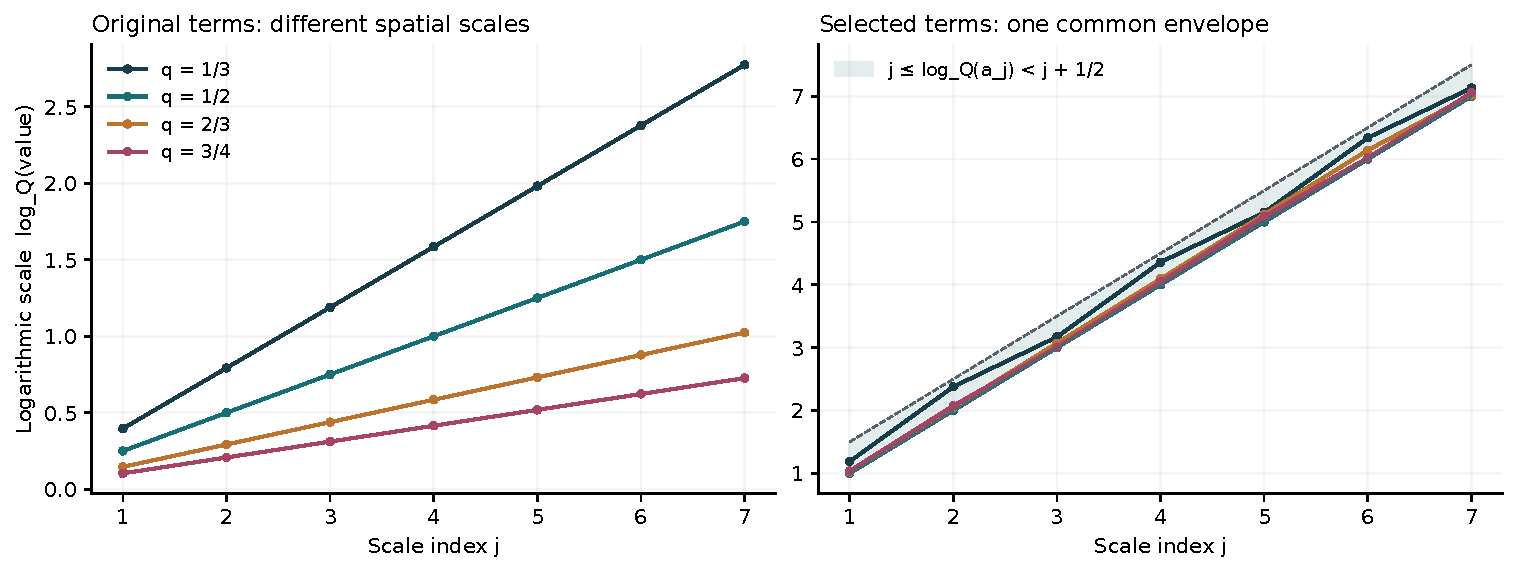
\includegraphics[width=\textwidth]{figures/synchronized_scales.pdf}
\caption{An exact sampling rule brings different ratios onto common scales.
The displayed example uses $Q=1/16$, $\alpha=1/4$, and four rational ratios.
On the right, the selected values satisfy
$j\le\log_Q a_j<j+1/2$, so the same spatial resolutions work for every
curve. The plot illustrates \cref{lem:envelopes}; the proof does not rely
on the finite set of ratios shown.}
\label{fig:sync}
\end{figure}

\subsection{One nested family of grids}

For integers $b\ge1$ choose
\begin{equation}\label{eq:grids}
 N_b=2^{\lceil\log_2(cQ^{-b})\rceil},\qquad
 \Gamma_b=N_b^{-1}\Z,\qquad
 J_b(z)=\lfloor N_b\{z\}\rfloor.
\end{equation}
Here $\{z\}$ is the fractional part. The cells are closed on the left
and open on the right, and
\begin{equation}\label{eq:grid-size}
 cQ^{-b}\le N_b<2cQ^{-b}.
\end{equation}
Since the $N_b$ are nondecreasing powers of two, every finer key determines
all coarser keys. This fact concerns actual periodic cells, including
cells adjacent to an integer.

\subsection{Preorder windows and their exact span}

Fix integers $M\ge2$, $d\ge1$, $g\ge1$, and $r_0\ge1$, to be chosen
in that order later. Let $\mathcal T$ be a complete ordered $M$-ary tree
of height $d$. Leaves have height zero. Write $P_i$ for the $i$th child
of $P$. An edge $e=(P,i)$ is listed immediately before all edges below
$P_i$, and that whole block precedes $(P,i+1)$. This is preorder.
Let
\begin{equation}\label{eq:Kedges}
 K=M+M^2+\cdots+M^d
\end{equation}
be the number of edges.

Each edge receives an integer window $W_e=[a_e,b_e]\cap\Z$.
Place the windows in preorder, with exactly $g$ unused indices between
successive windows. All edges from a height-$h$ vertex receive length
$r_h$. Define the subtree spans by
\begin{align}
 r_1&=r_0,& \sigma_1&=Mr_0+(M-1)g,\label{eq:window-recursion1}\\
 r_h&=g+\sigma_{h-1},&
 \sigma_h&=2M\sigma_{h-1}+(3M-1)g\quad(2\le h\le d).
 \label{eq:window-recursion2}
\end{align}
Every $r_h\ge r_0$. The expression for $\sigma_h$ counts $M$ blocks
consisting of an outgoing window, one gap, and its child subtree, together
with $M-1$ gaps between those blocks.

Start the first window at a fixed $j_0\ge1$ with $2Q^{j_0}\le1/4$.
Let
\begin{equation}\label{eq:B-global}
 B=j_0-1+\sigma_d,\qquad \mathcal J=\bigcup_e W_e.
\end{equation}
The letter $B$ always denotes this largest window index; the random set
will be denoted $A$.

For an edge $e$, let $b_e^*$ be the largest index in its own window or
any window in its child subtree.

\begin{lemma}[Local span and global affine growth]\label{lem:span}
If $e$ leaves a height-$h$ vertex, then
\begin{equation}\label{eq:span}
 b_e^*-a_e+1\le2r_h.
\end{equation}
For fixed $M,d,g,j_0$, the value $B$ is an affine function of $r_0$.
Explicitly,
\begin{align}
 \sigma_d={}&M(2M)^{d-1}r_0\notag\\
 &+\left((M-1)(2M)^{d-1}
 +(3M-1)\frac{(2M)^{d-1}-1}{2M-1}\right)g.
 \label{eq:affine-span}
\end{align}
\end{lemma}

\begin{proof}
For a leaf edge the span equals $r_1$. Otherwise preorder makes the
edge--subtree span exactly $r_h+g+\sigma_{h-1}=2r_h$.
Solving the affine recurrence \eqref{eq:window-recursion2}, starting
from \eqref{eq:window-recursion1}, gives \eqref{eq:affine-span}.
\end{proof}

The local bound \eqref{eq:span} controls the parameter count. The
separate global bound \eqref{eq:affine-span} ensures that polynomial
losses in $B$ can be absorbed by increasing $r_0$. Replacing every
local resolution by the finest grid of the entire tree would lose
this separation of roles.

\subsection{Stable centers and distinct addresses}

Call $x\in\R$ \emph{stable} if for every window except the first,
with $b'$ the endpoint of its immediate predecessor,
\begin{equation}\label{eq:stable-def}
 (x,x+2Q^{a_e}]\cap\Gamma_{b'}=\varnothing.
\end{equation}
Let $\calS$ be the stable set.

\begin{lemma}[Uniform stability]\label{lem:stable}
The set $\calS$ is measurable and $1$-periodic, and
\begin{equation}\label{eq:unstable-density}
 \rho(\R\setminus\calS)\le4KcQ^{g+1}.
\end{equation}
If $x\in\calS$, $j\in W_e$, $t\in[1,2]$, and
$q\in[\alpha,\beta]$, then every edge $f$ preceding $e$ satisfies
\begin{equation}\label{eq:earlier-key}
 J_{b_f}(x+ta_j(q))=J_{b_f}(x).
\end{equation}
\end{lemma}

\begin{proof}
The centers violating one condition in \eqref{eq:stable-def} lie in
$\bigcup_{\gamma\in\Gamma_{b'}}[\gamma-2Q^{a_e},\gamma)$.
Its density is at most $2N_{b'}Q^{a_e}<4cQ^{a_e-b'}=4cQ^{g+1}$.
A union bound over fewer than $K$ conditions proves
\eqref{eq:unstable-density}. For a stable center, the displacement
$ta_j(q)$ belongs to $(0,2Q^{a_e}]$, so it crosses no boundary of the
predecessor grid. A boundary at $x$ itself belongs to its right-hand
cell and causes no exception. Nestedness gives the assertion at every
earlier resolution.
\end{proof}

\begin{lemma}[Separation within a window]\label{lem:separation}
For every edge $e$ and every fixed $(x,t,q)$ in the stated ranges, the
points
\[
 \{x\}\cup\{x+ta_j(q):j\in W_e\}
\]
have pairwise distinct keys at resolution $b_e$ and at all finer
resolutions.
\end{lemma}

\begin{proof}
All points lie in an interval of length at most $2Q^{j_0}\le1/4$;
their ordinary distances therefore equal their circular distances.
Their distances from the center are greater than $\alpha Q^{b_e}$.
By \eqref{eq:sample-gap}, the distance between two translated points
is greater than $(\alpha-Q)Q^{b_e}$. But a cell has width at most
$Q^{b_e}/c=(\alpha-Q)Q^{b_e}/4$. Two points sharing a key have circular
distance less than that width. Thus the keys are distinct, and remain
so at finer resolutions.
\end{proof}

\section{Finite random routing and exact conditional failure}
\label{sec:routing}

This section presents the routing argument inherited from
\cite[Sections~3--4]{OpenAI84}, with the common grids and sampled terms
from \cref{sec:synchronization}. We include the conditioning details
because the points choose their leaves adaptively: unconditional
independence of their entire routes is neither true nor needed.

\subsection{Selectors, defaults, and terminal bits}

Set $m_0=M-1$. For every edge $e=(P,i)$ with $1\le i<M$, assign an
independent fair bit to every key at resolution $b_e$:
\[
 S_e:\{0,\ldots,N_{b_e}-1\}\longrightarrow\{0,1\}.
\]
The $M$th child is the default and has no selector table. For each
leaf $L$, let $b(L)$ be the endpoint of its incoming edge, and assign
independent Bernoulli-$p$ entries to a terminal table $T_L$ on the
keys at resolution $b(L)$. Every entry in all these tables is
independent of all others. The probability space is finite.

Route $z\in\R$ from the root. At each internal vertex choose the
first child $i<M$ for which $S_{(P,i)}(J_{b_{(P,i)}}(z))=1$;
if no such child exists, choose child $M$. Write $L(z)$ for the leaf
reached. Define the random set
\begin{equation}\label{eq:random-set}
 A=\{z:T_{L(z)}(J_{b(L(z))}(z))=1\}.
\end{equation}
Each realization is a $1$-periodic finite union of half-open cells.
All its tables and routing rules are independent of $q$ and $t$.

\begin{lemma}[Mean density]\label{lem:mean-density}
$\E\rho(A)=p$.
\end{lemma}

\begin{proof}
Let $\calA$ be the sigma-field of all selector entries. Conditional
on $\calA$, the terminal address of each fixed point $z$ is determined.
Its terminal bit remains Bernoulli-$p$, so
$\Prob(z\in A\mid\calA)=p$. Integrate on one period; since the
probability space is finite, the interchange of expectation and
integration is immediate.
\end{proof}

\subsection{Expose only the center entries}

For a fixed center $x$, reveal the addressed entry at $x$ in \emph{every}
selector table, including tables outside its route. Define
\begin{equation}\label{eq:center-field}
 \calF_x=\sigma\bigl(S_e(J_{b_e}(x)): e=(P,i),\ i<M\bigr)
 \subseteq\calA.
\end{equation}
The exposed addresses are deterministic. On any atom $\xi$ of $\calF_x$,
all other selector entries remain independent fair bits and all terminal
entries retain their independent Bernoulli-$p$ distributions.

At each vertex reached by $x$, its $m_0$ selector entries are fresh
relative to the previous ancestor decisions. Thus
\begin{equation}\label{eq:no-default}
 \Prob(\text{$x$ has no default on its route})=(1-2^{-m_0})^d.
\end{equation}
On an atom where the route uses a default, let $U$ be the first such
vertex and $h$ its height. Both are fixed on that atom. Put $r=r_h$
and $e_i=(U,i)$ for $1\le i\le m_0$. All selectors at $x$ on these
edges are zero.

For $z\in\R$, let $L_i(z)$ be the leaf reached by routing from
child $U_i$. Define a local test
\begin{equation}\label{eq:local-test}
 Q_i(z)=S_{e_i}(J_{b_{e_i}}(z))\,
 T_{L_i(z)}(J_{b(L_i(z))}(z)).
\end{equation}
This uses only the table on $e_i$ and tables below that child.

\begin{lemma}[A successful local test is an actual hit]\label{lem:local-hit}
Suppose $x\in\calS$ and the atom $\xi$ has first default $U$.
For $j\in W_{e_i}$ and any $q\in[\alpha,\beta]$, $t\in[1,2]$,
\begin{equation}\label{eq:local-hit}
 Q_i(x+ta_j(q))=1\quad\Longrightarrow\quad x+ta_j(q)\in A.
\end{equation}
\end{lemma}

\begin{proof}
At a strict ancestor of $U$, the child chosen by $x$ is nondefault.
Every selector consulted to make that choice lies earlier than $e_i$
in preorder. By \cref{lem:stable}, its value at $x+ta_j(q)$ equals
its value at $x$. Hence the translated point reaches $U$.
The selectors of children $1,\ldots,i-1$ of $U$ are also earlier
in preorder and remain zero. If the test in \eqref{eq:local-test}
is one, child $i$ is selected and its terminal entry is one. This is
exactly the membership rule \eqref{eq:random-set}.
\end{proof}

\begin{lemma}[Exact conditional failure]\label{lem:failure}
Under the assumptions of \cref{lem:local-hit}, for every fixed
$(q,t)\in[\alpha,\beta]\times[1,2]$,
\begin{equation}\label{eq:failure}
 \Prob\!\left(Q_i(x+ta_j(q))=0\text{ for every }i\le m_0,
 j\in W_{e_i}\,\middle|\,\xi\right)
 =(1-p/2)^{m_0r}.
\end{equation}
\end{lemma}

\begin{proof}
There are $m_0r$ pairs $(i,j)$. Write
\[
 A_{ij}=S_{e_i}(J_{b_{e_i}}(x+ta_j(q))).
\]
For one $i$, \cref{lem:separation} makes all these addresses distinct
and different from the exposed center address. Different $i$ use
different tables. Conditional on $\xi$, the $A_{ij}$ are therefore
independent fair bits.

Now condition on the larger sigma-field $\calA$ of \emph{all}
selectors. The leaf and terminal address of every local test are fixed.
Those addresses are pairwise distinct. Different children $i$ have
disjoint subtrees and hence different terminal tables. Within a child,
different leaves again have different tables. If two distinct $j,j'$
reach the same leaf, its resolution is at least $b_{e_i}$, so
\cref{lem:separation} makes their terminal keys distinct. This covers
all possible pairs.

Consequently, conditional on $\calA$, the probability that all tests
fail is
\[
 (1-p)^{\sum_{i,j}A_{ij}}.
\]
The tests with $A_{ij}=0$ already fail; each of the others consults a
different Bernoulli-$p$ terminal entry. Average this expression over
the independent fair $A_{ij}$ conditional on $\xi$:
\[
 \E\!\left[(1-p)^{\sum_{i,j}A_{ij}}\mid\xi\right]
 =\prod_{i,j}\left(\tfrac12+\tfrac12(1-p)\right)
 =(1-p/2)^{m_0r}.
\]
No independence of the internal routes has been invoked.
\end{proof}

The geometry now enters only through how many different vectors of
local keys can occur as $(q,t)$ varies. That count must be obtained
\emph{before} revealing the unexposed table entries; otherwise a
union bound over representatives would not be justified.

\section{A line arrangement controls every ratio and dilation}
\label{sec:uniformity}

Fix a stable center $x$ and an atom $\xi$ with first default vertex $U$.
Write $r=r_h$ for its window length. Every local test $Q_i(z)$ consults
only the edge $e_i=(U,i)$ and its child subtree. Thus its outcome, for
\emph{every} realization of the remaining tables, is determined by
$J_{b_{e_i}^*}(z)$. We count the possible vectors
\begin{equation}\label{eq:key-vector}
 \left(J_{b_{e_i}^*}(x+ta_j(q)):
  1\le i\le m_0,\ j\in W_{e_i}\right).
\end{equation}

\subsection{Counting all faces, not only open regions}

\begin{lemma}[An elementary arrangement bound]\label{lem:line-arrangement}
For $L$ affine lines in the plane, the total number of vertices,
one-dimensional faces, and two-dimensional faces is at most $2L^2+1$.
After restriction to a rectangle, the number of sign vectors of $F$
affine functions is therefore at most $2(F+4)^2+1$.
The same bound holds if either pair of opposite sides is omitted, and
is also an upper bound on a vertical segment.
\end{lemma}

\begin{proof}
Discard duplicate lines. There are at most $L(L-1)/2$ intersection
points. Each line is divided by at most $L-1$ points into at most $L$
one-dimensional open pieces, giving at most $L^2$ edges. Adding the
lines one at a time gives at most $1+L(L+1)/2$ two-dimensional regions.
The sum is $2L^2+1$. Parallel lines, multiple intersections, and other
degeneracies only reduce these bounds.
For a rectangle, append its four supporting lines. Every face of the
resulting arrangement has constant signs, including zeros. Its
intersection with the required rectangle or open-sided rectangle is
empty or a single convex face. On a vertical segment the direct bound
$2F+3$ is smaller than the stated bound.
\end{proof}

The inclusion of zero signs is essential: a point exactly on a cell
boundary belongs to its right-hand cell. Sampling only the interiors
of two-dimensional regions would not justify the construction.

\begin{lemma}[Deterministic parameter representatives]\label{lem:representatives}
Let
\begin{equation}\label{eq:F-count}
 F_r=m_0r(1+4cQ^{-2r}).
\end{equation}
The vector \eqref{eq:key-vector} has at most
\begin{equation}\label{eq:D-count}
 D(r,B)=(2Tm_0rB+3)\bigl[2(F_r+4)^2+1\bigr]
\end{equation}
possible values. In particular,
\begin{equation}\label{eq:D-coarse}
 D(r,B)\le C(B+1)^4Q^{-4r},
\end{equation}
where the constant independent of $r_0,r,B$ is
\begin{equation}\label{eq:C-count}
 C=(2T+3)\bigl[2(5+4c)^2+1\bigr]m_0^3.
\end{equation}
One representative $(q,t)$ for each value can be chosen using only
$x$, the deterministic grids and windows, and $U$; the unexposed random
entries are irrelevant to this choice.
\end{lemma}

\begin{proof}
There are $m_0r$ relevant indices $j$, all at most $B$.
Partition $[\alpha,\beta]$ at the jumps of every relevant
$\nu_j(q)$. Retain each jump and endpoint as a singleton, and each
intervening open interval as a separate stratum. By
\cref{lem:envelopes}, at most $2Tm_0rB+3$ strata result.
On an open stratum every exponent $n_j=\nu_j(q)$ is constant.

For a pair $(i,j)$, the translated point lies in $(x,x+2Q^j]$.
Only boundaries $\gamma\in\Gamma_{b_{e_i}^*}\cap[x,x+2Q^j]$
can change its key. Their number is at most
\begin{equation}\label{eq:boundary-count}
 1+2N_{b_{e_i}^*}Q^j
 \le1+4cQ^{j-b_{e_i}^*}
 \le1+4cQ^{-2r},
\end{equation}
using \cref{lem:span}. A boundary with $\gamma\le x$ is never
attained by a translated point and may be discarded. For the others,
the boundary equation is
\[
 tq^{n_j}=\gamma-x.
\]
In coordinates
\begin{equation}\label{eq:log-coordinates}
 u=-\log q,\qquad v=\log t,
\end{equation}
it becomes the affine line
\begin{equation}\label{eq:boundary-line}
 v-n_ju=\log(\gamma-x).
\end{equation}
There are at most $F_r$ such lines, counting repetitions if necessary.
The logarithm is increasing, so its sign relative to a boundary is
exactly the sign of the original displacement relative to that boundary.
The sign vector, including its zeros, determines every key in
\eqref{eq:key-vector}.

On an open ratio stratum, \cref{lem:line-arrangement} supplies at most
$2(F_r+4)^2+1$ representatives. On a singleton stratum the exponents
are assigned by \eqref{eq:nu}, and a one-dimensional boundary count
gives the same upper bound. Multiplication by the number of strata
proves \eqref{eq:D-count}. All geometric data used here are fixed
under $\xi$.

Finally $r\le B$, $m_0\ge1$, and $Q^{-2r}\ge1$. Hence
\[
 2Tm_0rB+3\le(2T+3)m_0(B+1)^2,
 \qquad
 F_r+4\le m_0r(5+4c)Q^{-2r}.
\]
These inequalities give \eqref{eq:D-coarse} with \eqref{eq:C-count}.
\end{proof}

\begin{proposition}[Conditional uniform failure bound]\label{prop:uniform-failure}
For a stable $x$ and an atom $\xi$ whose first default has height $h$,
\begin{align}
 &\Prob\!\left(\exists(q,t)\in[\alpha,\beta]\times[1,2]
   \ \forall j\in\mathcal J:\ x+ta_j(q)\notin A
   \,\middle|\,\xi\right)\notag\\
 &\hspace{30mm}\le C(B+1)^4
  \bigl[Q^{-4}(1-p/2)^{m_0}\bigr]^{r_h}.
 \label{eq:uniform-failure}
\end{align}
\end{proposition}

\begin{proof}
If the selected points all miss $A$, \cref{lem:local-hit} implies
failure of all local tests at that parameter pair. A representative
from \cref{lem:representatives} has exactly the same key vector, so
all its local tests also fail for that realization of the tables.
Apply \cref{lem:failure} at each representative, and then the union
bound and \eqref{eq:D-coarse}. Because representatives were selected
before revealing the remaining entries, each application uses precisely
the fixed-parameter probability proved in \cref{lem:failure}.
\end{proof}

\subsection{Choose the parameters without a circular dependence}

Here is the complete order of choice.
First, after fixing $p,\alpha,\beta,Q,T,c$, choose $M$ so large that
\begin{equation}\label{eq:theta}
 \theta=Q^{-4}(1-p/2)^{M-1}<1.
\end{equation}
Second choose $d$ with $(1-2^{1-M})^d<p$.
Third compute $K$ from \eqref{eq:Kedges} and choose $g$ with
\begin{equation}\label{eq:gap-choice}
 4KcQ^{g+1}<p.
\end{equation}
The index $j_0$ was fixed using only $Q$.
Finally choose $r_0$ so large that
\begin{equation}\label{eq:base-length-choice}
 C(B(r_0)+1)^4\theta^{r_0}<p.
\end{equation}
Such a choice exists because \cref{lem:span} makes $B(r_0)$ affine
in $r_0$ while $0<\theta<1$. For every height $h$ we have
$r_h\ge r_0$, so \eqref{eq:uniform-failure} is less than $p$ with
this same choice. All comparisons in the choices can be made with
rational arithmetic when the initial parameters are rational.

Together with \eqref{eq:no-default}, this proves, for every stable $x$,
\begin{equation}\label{eq:pointwise-miss}
 \Prob\!\left(\exists(q,t)\in[\alpha,\beta]\times[1,2]
  \ \forall j\in\mathcal J:\ x+ta_j(q)\notin A\right)<2p.
\end{equation}
No claim is made that the required tree is of manageable size. The
parameter choice proves existence; its computational cost is discussed
in \cref{sec:effective}.

\subsection{Repair all centers using the original exponents}

We now prove \cref{prop:normalized}. For each table outcome, enlarge
the finite half-open cell union $A$ to an open periodic $A^+\supset A$
with $\rho(A^+)\le\rho(A)+p$. Define
\begin{equation}\label{eq:R-original}
 R=\left\{x\in\R:\exists(q,t)\in[\alpha,\beta]\times[1,2]
   \quad x+tq^n\notin A^+\ \text{for all }1\le n\le TB\right\}.
\end{equation}
The use of the \emph{original} exponents in this definition is deliberate.
The maps $q\mapsto a_j(q)$ jump. A projection argument applied directly
to those selected terms would not establish closedness.

By contrast, $x+tq^n$ is continuous for every original integer $n$.
On $(\R/\Z)\times[\alpha,\beta]\times[1,2]$ the joint miss set
in \eqref{eq:R-original} is closed. Its projection $R$ is therefore
closed and periodic. If a stable center belongs to $R$, then for the
witnessing $(q,t)$ all selected exponents also miss, because
$\nu_j(q)\le Tj\le TB$. Thus \eqref{eq:pointwise-miss} bounds
$\Prob(x\in R)$ by $2p$ on $\calS$. From
\eqref{eq:unstable-density} and \eqref{eq:gap-choice},
\begin{equation}\label{eq:expected-R}
 \E\rho(R)\le2p\rho(\calS)+\rho(\R\setminus\calS)\le3p.
\end{equation}
Also \cref{lem:mean-density} gives $\E\rho(A^+)\le2p$.
Choose an outcome with
\[
 \rho(A^+)+\rho(R)\le5p.
\]
Outer regularity on the circle supplies an open periodic $V\supset R$
with $\rho(V)\le\rho(R)+p$. Set $H=A^+\cup V$. Then
$\rho(H)\le6p$.

For $x\notin R$, every pair $(q,t)$ has a hit in $A^+$ among
$n=1,\ldots,TB$. For $x\in R$, openness of $V$ and convergence
$x+tq^n\to x$ give a hit in $V$ for all sufficiently large $n$.
This proves \eqref{eq:normalized-hit}, and hence
\cref{prop:normalized}. Notice that the repair indices need not lie
in the finite prefix used to define $R$.

\section{A common periodic set and consequences}
\label{sec:global}

\subsection{Only contracting copies of the periodic sets are needed}

We prove \cref{thm:main}. For $j\ge1$ put
\begin{equation}\label{eq:ratio-exhaustion}
 I_j=\left[\frac1{j+2},1-\frac1{j+2}\right],
 \qquad \bigcup_{j\ge1}I_j=(0,1).
\end{equation}
For $j\ge1$ and $k\ge0$, use \cref{prop:normalized} on $I_j$ with
\begin{equation}\label{eq:global-budget}
 p_{j,k}=\frac\eps{24}\,2^{-j}2^{-(k+1)}
\end{equation}
to obtain $H_{j,k}$. Define
\begin{equation}\label{eq:global-C}
 C=\bigcup_{j\ge1,\ k\ge0}
 \left(2^{-k}H_{j,k}\ \cup\ (-2^{-k}H_{j,k})\right),
 \qquad F_\eps=\R\setminus C.
\end{equation}
Every component in this union is open with period $2^{-k}$ and hence
also period one. The union is open, symmetric, and $1$-periodic.
The density of a contracted component in a unit interval is
\begin{equation}\label{eq:contraction-density}
 \rho(2^{-k}H_{j,k})=\rho(H_{j,k}).
\end{equation}
It is \emph{not} $2^{-k}\rho(H_{j,k})$: there are $2^k$ complete
periods in a unit interval. The summable budget explicitly pays for
this fact. Reflections have the same density, and therefore
\begin{equation}\label{eq:global-density}
 \rho(C)\le12\sum_{j\ge1,k\ge0}p_{j,k}=\frac\eps2.
\end{equation}
Periodicity gives \eqref{eq:main-density} for every $u$.

Fix $x$, $s\ne0$, and $q\in(0,1)$, and choose $j$ with $q\in I_j$.
Choose an integer $h\ge0$ so that $0<|s|q^h\le1$.
There are $k\ge0$ and $t\in[1,2)$ with
\begin{equation}\label{eq:tail-normalization}
 |s|q^h=2^{-k}t.
\end{equation}
If $s>0$, apply the normalized hitting property of $H_{j,k}$ at center
$2^kx$. Some $n\ge1$ satisfies
\[
 2^kx+tq^n\in H_{j,k},
 \quad\text{so}\quad x+sq^{h+n}\in2^{-k}H_{j,k}\subset C.
\]
If $s<0$, apply it at $-2^kx$ and reflect; the hit lies in
$-2^{-k}H_{j,k}$. This proves that every orbit meets $C$.
Apply the same assertion after any initial tail, replacing $s$ by
$sq^J$, to obtain arbitrarily late hits. The proof of
\cref{thm:main} is complete.

This contraction-only assembly improves the global organization of
the fixed-ratio construction. It uses the elementary identity that a
tail of $G_q$ is a scaled copy of $G_q$. It does not require a relation
between the ratio $q$ and the dyadic grid base.

\subsection{Large compact subsets of arbitrary measurable sets}

\begin{corollary}[Avoidance inside any measurable set]\label{cor:inside}
If $A\subset\R$ is measurable with $0<m(A)<\infty$, then for every
$\delta>0$ there is a compact $K\subset A$ such that
$m(K)>m(A)-\delta$ and $K$ contains no affine copy of any $G_q$,
$0<q<1$.
\end{corollary}

\begin{proof}
Choose compact $A_0\subset A$ with $m(A_0)>m(A)-\delta/2$ and a
bounded interval $I$ containing $A_0$. An affine image of the compact
set in \cref{thm:main}, with sufficiently small accuracy, gives a
compact $K_0\subset I$ with $m(I\setminus K_0)<\delta/2$.
Set $K=A_0\cap K_0$. Avoidance is inherited by subsets and preserved
by invertible affine maps; the measure bound follows.
\end{proof}

\begin{corollary}[A fat Cantor avoiding set]\label{cor:fat-cantor}
The compact set in \cref{thm:main} can be chosen perfect and nowhere
dense without losing measure. In particular there is a fat Cantor
set answering \cite[Question~1]{BGKMW} negatively.
\end{corollary}

\begin{proof}
The set $F_\eps$ has empty interior, since every nonempty interval
contains an affine contracting geometric progression. Its compact
section $K$ is therefore nowhere dense. Let $K'$ be the support of
the finite measure $\ind_K\,dm$. It is a closed subset of $K$;
its complement in $K$ is covered by countably many rational intervals
of that measure zero, so $m(K')=m(K)$. The support has no isolated
points: a measure supported on one isolated point of a neighborhood
would have an atom there, whereas $\ind_K\,dm$ is atomless.
Thus $K'$ is perfect and has all the required properties.
\end{proof}

The effective-closedness claim later concerns the original construction.
We do not infer an effective procedure for taking the measure support
in \cref{cor:fat-cantor}.

\begin{corollary}[Finite-dimensional line patterns]\label{cor:dimensions}
For each $d\ge1$ and $\delta>0$, there is a compact
$E\subset[0,1]^d$ of $d$-dimensional measure greater than $1-\delta$
containing no set $\{x+q^nv:n\ge1\}$ with $x\in\R^d$,
$v\in\R^d\setminus\{0\}$, and $0<q<1$.
\end{corollary}

\begin{proof}
Take $E=K^d$ with $m(K)$ sufficiently close to one. A nonzero $v$
has a nonzero coordinate. Projection to that coordinate would give
an affine copy of $G_q$ in $K$ if the whole pattern lay in $E$.
\end{proof}

The periodic set in \cref{thm:main} is asserted to avoid contracting
ratios. A nonempty periodic set cannot exclude all expanding geometric
orbits: it contains $x+2^n$ whenever it contains $x$. The compact
section automatically excludes expanding orbits because they are
unbounded. The range $0<q<1$ keeps the main statement precise.

\section{Polynomial families and finite exponential mixtures}
\label{sec:algebraic}

The geometric proof works because the dependence of all selected terms
on the parameters has controlled complexity. For a fixed-dimensional
polynomial family, a classical sign-condition theorem provides that
control even when the degrees grow with the original sequence index.
We state the general normalized result first. No semialgebraicity of
the parameter set is needed for this existence theorem.

\begin{theorem}[Uniform hitting for polynomial families]\label{thm:poly-family}
Let $\Theta\subset\R^d$ be nonempty and compact, and let
$f_n\in\R[X_1,\ldots,X_d]$, $n\ge0$, satisfy $f_0=1$ on $\Theta$.
Suppose there are constants $0<\alpha<\beta<1$, $A_0\ge1$, and
an integer $D_0\ge1$ such that, for all $n\ge0$ and $z\in\Theta$,
\begin{equation}\label{eq:family-assumptions}
 \alpha f_n(z)\le f_{n+1}(z)\le\beta f_n(z),
 \qquad \deg f_n\le A_0(n+1)^{D_0}.
\end{equation}
For each $0<p<1$ there exists an open $1$-periodic $H\subset\R$
with $\rho(H)\le6p$ such that
\begin{equation}\label{eq:family-hit}
 \forall x\in\R\ \forall t\in[1,2]\ \forall z\in\Theta
 \quad \exists n\ge1:\ x+tf_n(z)\in H.
\end{equation}
\end{theorem}

By induction, $\alpha^n\le f_n(z)\le\beta^n$, so every member
is strictly positive, strictly decreasing, and converges uniformly to
zero. The family may contain coinciding members and redundant
parameters.

\subsection{The sign-condition theorem used}

\begin{lemma}[Classical full sign-condition bound]\label{lem:signs}
If $S$ real polynomials in $v\ge1$ variables have degrees at most
$\Delta\ge1$, then the number of realized sign vectors in
$\{-1,0,1\}^S$ is at most
\begin{equation}\label{eq:sign-bound}
 \bigl(8\Delta(S+1)\bigr)^v.
\end{equation}
The same bound holds after restricting the variables to an arbitrary
subset of $\R^v$.
\end{lemma}

\begin{proof}[Justification and source]
We use the finite all-sign-condition component bound recorded in
\cite[Section~3.2, equation~(3.3)]{BPR}, with ambient dimension $v$:
\[
 \#\{\text{realized sign vectors}\}
 \le \sum_{j=0}^v\binom Sj4^j\Delta(2\Delta-1)^{v-1}.
\]
A sign realization has at least one connected component, so that
component estimate implies the displayed inequality. Since
$\binom Sj\le S^j$ and
$\sum_{j=0}^v(4S)^j\le(1+4S)^v$, the right-hand side is at most
$2^{v-1}\Delta^v(1+4S)^v\le(8\Delta(S+1))^v$.
Restriction cannot increase the number of realized sign vectors.
This is a finite degree-dependent bound, not just a fixed-degree
asymptotic. It includes zero signs.
\end{proof}

We do not need to distinguish connected components with the same sign
vector: the vector itself determines all the discrete choices below.
This observation also allows an arbitrary compact $\Theta$ in
\cref{thm:poly-family}.

\subsection{Simultaneously encode selection and grid addresses}

Choose $Q,T,c$ as in \eqref{eq:Q-T} and define, for $z\in\Theta$,
\[
 \nu_j(z)=\min\{n\ge1:f_n(z)\le Q^j\},
 \qquad a_j(z)=f_{\nu_j(z)}(z).
\]
Exactly as in \cref{lem:envelopes},
\begin{equation}\label{eq:family-envelope}
 \alpha Q^j<a_j(z)\le Q^j,\quad \nu_j(z)\le Tj,
 \quad a_j(z)-a_{j'}(z)>(\alpha-Q)Q^j\quad(j'>j).
\end{equation}
Thus the common grids, windows, stable centers, and finite random
routing from \cref{sec:synchronization,sec:routing} apply without
change. In particular the fixed-$(z,t)$ failure probability is
$(1-p/2)^{m_0r}$.

Fix $x$ and a center-exposure atom with first default $U$.
There are $m_0r$ relevant pairs $(i,j)$. Put $N=TB$.
For every relevant $j$ and $1\le n\le N$, include the polynomial
\begin{equation}\label{eq:selection-polynomial}
 f_n(z)-Q^j.
\end{equation}
The signs of these polynomials, including equality, determine the
first $n$ at which the level is crossed, and hence determine
$\nu_j(z)$.

For every pair $(i,j)$, each grid boundary
\[
 \gamma\in\Gamma_{b_{e_i}^*}\cap[x,x+2Q^j],
\]
and every $1\le n\le N$, also include
\begin{equation}\label{eq:key-polynomial}
 t f_n(z)-(\gamma-x).
\end{equation}
There are at most $1+4cQ^{-2r}$ such boundaries per pair by
\eqref{eq:boundary-count}. Some of the resulting tests are irrelevant
when $n$ is not selected; retaining them only enlarges the bound.
Once \eqref{eq:selection-polynomial} specifies $\nu_j(z)$, the signs
in \eqref{eq:key-polynomial} for that $n$ determine the selected
point's key. All selected points lie in the interval used to list
the boundaries, by \eqref{eq:family-envelope}.

The combined list contains at most
\begin{equation}\label{eq:family-S}
 S\le m_0rTB\bigl(2+4cQ^{-2r}\bigr)
\end{equation}
polynomials in $v=d+1$ variables $(z,t)$, of degrees at most
\begin{equation}\label{eq:family-degree}
 \Delta\le A_0(TB+1)^{D_0}+1.
\end{equation}
A realized sign vector determines the full local key vector for every
unrevealed table outcome. Representatives can therefore be chosen
before those entries are revealed, exactly as in the geometric proof.
By \cref{lem:signs}, \eqref{eq:family-S}, and
\eqref{eq:family-degree}, their number is at most
\begin{equation}\label{eq:family-complexity}
 C_0(B+1)^{(D_0+2)v}Q^{-2vr},
\end{equation}
where $C_0$ depends on $d,A_0,D_0,T,c,M$, but not on $r_0,r,B$.
Here we used $r\le B$ and absorbed only polynomial factors into
$(B+1)^{(D_0+2)v}$.

\subsection{Complete the normalized family proof}

Choose $M$ so that
\begin{equation}\label{eq:family-theta}
 \theta_v=Q^{-2v}(1-p/2)^{M-1}<1.
\end{equation}
Then choose $d_{\rm tree}$ (the tree height, distinct from parameter
dimension $d$), followed by $g$, so that the no-default probability
and the unstable-center density are each less than $p$.
With these choices fixed, $B(r_0)$ is affine in $r_0$.
Choose $r_0$ large enough that
\[
 C_0(B(r_0)+1)^{(D_0+2)v}\theta_v^{r_0}<p.
\]
The union bound over the representatives now gives the same pointwise
stable-center estimate as \eqref{eq:pointwise-miss}, uniformly for
$(z,t)\in\Theta\times[1,2]$.

Enlarge the random set to $A^+$ and define the residual centers by
\[
 R=\{x:\exists(z,t)\in\Theta\times[1,2],\ 
       x+tf_n(z)\notin A^+\text{ for every }1\le n\le TB\}.
\]
This is closed and periodic because the original polynomials are
continuous and $\Theta\times[1,2]$ is compact. Its expected density
is at most $3p$. The identical open-neighborhood repair gives an open
periodic $H$ of density at most $6p$. On a residual center the original
terms converge to the center, uniformly because $f_n\le\beta^n$.
This proves \cref{thm:poly-family}.

\subsection{Proof for all positive mixtures}

Fix a component count $d\ge1$ and an interval $I_j=[\alpha_j,\beta_j]$
from \eqref{eq:ratio-exhaustion}. Take
\begin{equation}\label{eq:mixture-family}
 \Theta_{d,j}=\{w\in[0,1]^d:\textstyle\sum_iw_i=1\}\times I_j^d,
 \qquad f_n(w,q)=\sum_{i=1}^d w_iq_i^n.
\end{equation}
This is a compact rational semialgebraic parameter set. The polynomials
have degree at most $n+1$, $f_0=1$, and
\[
 \alpha_j f_n(w,q)\le f_{n+1}(w,q)\le\beta_j f_n(w,q).
\]
Thus \cref{thm:poly-family} applies. There is no loss at repeated bases
or zero weights, since all arguments include boundary sign conditions.

Enumerate the pairs $(d,j)$ by $\ell\ge1$ in a computable order.
For each $\ell,k$, with $k\ge0$, choose the normalized blocker for
that family with budget
\[
 p_{\ell,k}=\frac\eps{24}2^{-\ell}2^{-(k+1)}.
\]
Form $C^*$ by the same union of signed contractions as
\eqref{eq:global-C}, and put $F^*_\eps=\R\setminus C^*$.
It is closed, symmetric, periodic, and has density at least $1-\eps/2$.

It remains to verify that a tail can always be brought back into one
of the normalized families. Absorb $\sum_i c_i$ into the dilation,
so assume $\sum_i c_i=1$ and write $a_n=\sum_i c_iq_i^n$.
For $h\ge0$ set
\begin{equation}\label{eq:mixture-tail}
 w_i^{(h)}=\frac{c_iq_i^h}{a_h},
 \qquad
 a_{h+n}=a_h\sum_i w_i^{(h)}q_i^n.
\end{equation}
The new weights remain in the same simplex. Choose $h$ large enough
that $|s|a_h\le1$, then normalize it by a dyadic contraction as in
\eqref{eq:tail-normalization}. The appropriate normalized blocker
gives a hit at an original index $h+n$. Since $h$ can be required to
exceed any prescribed threshold, the hits occur infinitely often.
This proves \cref{thm:mixtures}.

\subsection{An additional class: positive polynomial factors}

\begin{corollary}[Positive exponential polynomials]\label{cor:exp-polynomial}
One common closed, symmetric, $1$-periodic set of measure greater than
$1-\eps$ per unit interval can avoid, with infinitely many omissions,
every nontrivial affine pattern whose terms are
\begin{equation}\label{eq:positive-exp-poly}
 a_n=\sum_{i=1}^d P_i(n)q_i^n,
 \qquad 0<q_i<1,
\end{equation}
where $d$ is finite and the $P_i$ have nonnegative real coefficients,
not all zero. The compact section can also have the effective properties
of \cref{thm:effective-intro}.
\end{corollary}

\begin{proof}
Fix $d$, a degree bound $D$, a base interval $[\alpha,\beta]=I_j\subset(0,1)$,
and an integer $h\ge1$ so large that
$\beta(1+1/h)^D<1$. Consider normalized families
\[
 f_n(w,q)=\sum_{i=1}^d\sum_{k=0}^D
    w_{ik}(1+n/h)^kq_i^n,
 \quad w_{ik}\ge0,\quad\sum_{i,k}w_{ik}=1,
 \quad q_i\in[\alpha,\beta].
\]
They have $f_0=1$ and polynomial parameter degree at most $n+1$.
Each summand's ratio from $n$ to $n+1$ lies between $\alpha$ and
$\beta(1+1/h)^D<1$, and so does the ratio of the sums. Apply
\cref{thm:poly-family}, and assemble blockers over all the countably
many choices of $d,D,j,h$, with summable budgets.

Write $P_i(n)=\sum_k c_{ik}n^k$, $c_{ik}\ge0$. A tail has
\[
 a_{h+n}=A_h\sum_{i,k}w_{ik}^{(h)}(1+n/h)^kq_i^n,
 \quad
 A_h=\sum_{i,k}c_{ik}h^kq_i^h,
 \quad w_{ik}^{(h)}=\frac{c_{ik}h^kq_i^h}{A_h}.
\]
For all $h\ge1$, $A_h>0$; it tends to zero as $h\to\infty$.
Choose $h$ satisfying the contraction condition and $|s|A_h\le1$,
and as large as desired. The normalized family and a dyadic contraction
then produce an arbitrarily late hit. The families have effective
rational polynomial descriptions; the argument of
\cref{sec:effective} therefore applies.
\end{proof}

In \cref{cor:exp-polynomial}, negative polynomial coefficients and
complex bases are outside that corollary. The next theorem removes the
coefficient restriction by proving a separate uniform tail reduction.

\subsection{Signed coefficients and stable positive-root recurrences}

The positivity restriction can in fact be removed when every base is a
positive real number. The price is a countable compact exhaustion that
controls the dominant term before the normalized theorem is applied.

\begin{theorem}[All real exponential polynomials with positive bases]
\label{thm:signed-exp-poly}
For every $0<\eps<1$ there exists one closed, symmetric, $1$-periodic
set $F^{\rm ep}_\eps\subset\R$, of measure at least $1-\eps/2$ in
every unit interval, with the following property. For every finite sum
\begin{equation}\label{eq:signed-exp-poly}
 A_n=\sum_{i=1}^m P_i(n)q_i^n,\qquad q_i\in(0,1),
\end{equation}
with arbitrary real polynomial coefficients, not identically zero
after equal bases have been combined, and every $x\in\R$, $s\ne0$,
infinitely many $x+sA_n$ lie outside $F^{\rm ep}_\eps$.
For rational accuracy its compact section can be effectively closed
with computable measure.
\end{theorem}

\begin{proof}
Combine equal bases and discard zero polynomials. Relabel so that
$q_m$ is the largest remaining base. If $P_m$ has degree $j$ and
nonzero leading coefficient $\lambda$, divide all polynomials by
$\lambda$ and replace $s$ by $s\lambda$. Hence we may suppose
$P_m$ is monic of degree $j$.

Fix integers $m\ge1$, $k\ge j\ge0$, $R\ge1$, and rational
$0<a<b<1$, $0<\delta<b$. Consider the compact parameter set where
all bases belong to $[a,b]$, all polynomial degrees are at most $k$,
all coefficients have absolute value at most $R$, $P_m$ is monic of
degree $j$, and
\[
 q_i\le q_m-\delta\quad(i<m).
\]
For $m=1$ the separation conditions are vacuous. The set is rational
semialgebraic. Empty sets may be skipped by quantifier elimination.
Countably many such boxes cover every normalized nonzero expression.

Put $r_*=1-\delta/b\in(0,1)$. Uniformly on each box, for $n\ge1$,
\begin{equation}\label{eq:dominance}
 A_n=n^jq_m^n(1+E_n),\qquad
 |E_n|\le \frac{Rj}{n}+(m-1)R(k+1)n^k r_*^n.
\end{equation}
Indeed the lower terms of the monic dominant polynomial contribute
at most $Rj/n$ after division by $n^j$. Each other polynomial has
absolute value at most $R(k+1)n^k$, and its base ratio is at most
$1-\delta/q_m\le1-\delta/b=r_*$. Dropping the additional factor
$n^{-j}\le1$ gives the stated estimate.

Choose rational $e\in(0,1)$ such that $b(1+e)/(1-e)<1$.
Then choose $N$ large enough that the right-hand side of
\eqref{eq:dominance} is at most $e$ for every $n\ge N$ and
\[
 \beta_*:=b(1+1/N)^j\frac{1+e}{1-e}<1.
\]
These choices are effective: after imposing
$(1+1/N)^kr_*\le r'_*<1$ for some rational $r'_*\in(r_*,1)$,
the sequence $n^kr_*^n$ is decreasing for $n\ge N$, so the
required tail bounds reduce to rational inequalities at $N$.
It follows that $A_n>0$ for $n\ge N$, and
\begin{equation}\label{eq:dominant-ratios}
 \alpha_*:=a\frac{1-e}{1+e}
 \le\frac{A_{n+1}}{A_n}\le\beta_*<1
 \qquad(n\ge N).
\end{equation}

For \emph{each} integer $h\ge N$, augment this compact box by the
parameter $u$ satisfying $uA_h=1$, and use the sequence of polynomials
\[
 f_n=uA_{h+n},\qquad n\ge0.
\]
The augmented set is compact: $A_h\ge(1-e)h^j a^h>0$ uniformly,
so $u=1/A_h$ is continuous and bounded there. It is rational
semialgebraic, $f_0=1$, and \eqref{eq:dominant-ratios} gives the
required uniform contraction bounds. Parameter degree is at most
$h+n+2$, so \cref{thm:poly-family} applies.

Enumerate all these boxes \emph{and all integers $h\ge N$} as the
normalized families in the signed-contraction assembly of
\cref{sec:global}. The same budgets give one periodic set of density
at least $1-\eps/2$. For any original expression, choose its box and
then $h$ as large as desired with $|s|A_h\le1$. Since
$A_{h+n}=A_h f_n$, a dyadic contraction of the normalized blocker
hits the original affine sequence at an index beyond $h$.
This proves infinitely many omissions. Including every $h\ge N$
is what makes the contractions-only assembly valid for these
normalized tail families.

All enumerated families and tail bounds have effective rational data.
Consequently \cref{prop:effective-H} and the measure modulus in
\cref{sec:effective} prove the last assertion.
\end{proof}

\begin{corollary}[Real linear recurrences with roots in $(0,1)$]
\label{cor:recurrences}
The set $F^{\rm ep}_\eps$ simultaneously avoids, with infinitely many
omissions in every nonzero affine scale, every nonzero real solution of a
homogeneous constant-coefficient linear recurrence whose characteristic
roots are all real and lie in $(0,1)$, allowing repeated roots.
\end{corollary}

\begin{proof}
For completeness, if the distinct roots are $q_i$ with multiplicities
$m_i$, the sequences $n^kq_i^n$, $0\le k<m_i$, satisfy the recurrence.
Applying the shift operator minus $q_i$ lowers the polynomial degree
in the corresponding term. These $\sum_i m_i$ sequences are linearly
independent: in a vanishing combination, divide by the largest base
to isolate its polynomial, which cannot tend to zero unless it is
zero; then repeat for the smaller bases. A recurrence of order
$\sum_i m_i$ has that dimension of solutions, since its initial
values determine it. Therefore every solution has the form
\eqref{eq:signed-exp-poly}. A nonzero solution gives a nonzero
expression, and \cref{thm:signed-exp-poly} applies.
\end{proof}

\section{Effective closed sets and finite avoidance certificates}
\label{sec:effective}

The existence proof uses finite but extremely large random tables.
It also uses real parameters and an open-neighborhood repair.
Nevertheless, the resulting compact sets can be made effective by
searching directly for finite certificates. This route avoids having
to implement the entire probabilistic construction.

\subsection{A finite rational normalized certificate}

A \emph{rational periodic open set} is a finite union of rational open
arcs on $\R/\Z$, lifted periodically to $\R$. Its density is a
computable rational number, obtained by merging the arcs on one period.
An arc crossing zero is represented by an interval $(a,b)$ with
$0\le a<1$ and $a<b\le a+1$, together with its integer translates.
Dyadic rational endpoints suffice.

\begin{proposition}[Terminating search for normalized blockers]\label{prop:effective-H}
Given rational $0<\alpha<\beta<1$ and rational $0<p<1$, there is an algorithm
that returns a rational periodic open set $H$ and an integer $N\ge1$
such that $\rho(H)<6p$ and
\begin{equation}\label{eq:finite-H}
 \forall x\in[0,1]\ \forall t\in[1,2]\ \forall q\in[\alpha,\beta]
 \quad \bigvee_{n=1}^{N}(x+tq^n\in H).
\end{equation}
The analogous statement holds for a rational semialgebraic compact
parameter set and a computably given sequence of rational polynomials
satisfying \cref{thm:poly-family}. These hypotheses are promises;
the algorithm need not decide them from an arbitrary infinite sequence.
\end{proposition}

\begin{proof}
Enumerate pairs $(H,N)$ consisting of finite dyadic open arc unions
and positive integers, in an order eventually reaching every pair.
Discard candidates with density at least $6p$. For each remaining
candidate, decide \eqref{eq:finite-H} by quantifier elimination in
the ordered real field. The expressions $x+tq^n$ are polynomials with
rational coefficients. They lie in $[0,3]$, so membership in $H$
is a finite disjunction over only finitely many integer translates
of its arcs. The entire formula is therefore a first-order sentence
about rational polynomial inequalities. Real quantifier elimination
is effective; see, for example, \cite{PerrucciRoy}.

To prove termination, apply \cref{prop:normalized} with $p/2$,
obtaining an open periodic $H_0$ of density at most $3p$.
For each point of the compact parameter box there is a witnessing
integer $n$ and a small open interval, with dyadic endpoints, containing
the witnessing value and contained in $H_0$. By continuity of the
original expression, the same interval and exponent work on a
neighborhood of that parameter point. Finitely many of these
neighborhoods cover the compact box. Their finitely many witnessing
intervals project to a rational periodic open subset $H$ of $H_0$;
let $N$ be the largest witnessing exponent. Then
$\rho(H)\le3p<6p$ and \eqref{eq:finite-H} holds. Hence the search
must encounter a valid pair.

For polynomial families, replace $q^n$ by $f_n(z)$ and include the
rational semialgebraic formula defining $\Theta$ in the quantified
domain. Continuity, compactness, and effective real polynomial
arithmetic give the same proof.
\end{proof}

This is a proof of a total algorithm on the stated inputs, not a
reported computation of the full hitting set. The certificate search
may be enormous. A more direct implementation could enumerate the
finite tables, eliminate the residual-center quantifiers, and isolate
algebraic endpoints, but no such implementation is required for the
effective existence result.

\subsection{A computable measure modulus}

Use \cref{prop:effective-H} for every normalized family in the global
assembly. Index the families by $\ell\ge1$: this can mean the intervals
$I_\ell$ for the geometric theorem, the pairs $(d,j)$ for mixtures,
or the tuples used in \cref{cor:exp-polynomial,thm:signed-exp-poly}. In each case there
is a computable enumeration of rational semialgebraic families with
computably given rational polynomials. Use
\[
 p_{\ell,k}=\frac\eps{24}2^{-\ell}2^{-(k+1)}
 \quad(\ell\ge1,\ k\ge0).
\]
For $N\ge1$, let $C_N$ contain precisely the signed contractions with
$1\le\ell\le N$ and $0\le k<N$, and set
\begin{equation}\label{eq:KN}
 K_N=[0,1]\setminus C_N.
\end{equation}
The set $K_N$ is a computable finite union of closed rational intervals,
and the sequence is nested. The omitted density budget is bounded by
\begin{align}
 m(K_N)-m(K)
 &\le12\sum_{\ell>N\ \mathrm{or}\ k\ge N}p_{\ell,k}\notag\\
 &=\frac\eps2\left[1-(1-2^{-N})^2\right]
 \le\eps\,2^{-N}.
 \label{eq:measure-modulus}
\end{align}
Here the sums are over the union of the two omitted index ranges;
the overlap is not counted twice. This proves
\eqref{eq:effective-rate-intro}. Since $m(K_N)$ is rational and its
error has the computable bound \eqref{eq:measure-modulus}, $m(K)$
is a computable real. The same enumeration of rational intervals
shows that $K$ is effectively closed relative to $[0,1]$, and hence
as a compact subset of $\R$ after including its exterior in the
open complement.

A different rational accuracy can be computed independently. No
uniform operation on an unspecified noncomputable real $\eps$ is
asserted. For a nonrational positive accuracy, the existence statements
follow by choosing a smaller rational accuracy.

\subsection{Finite prefixes with a positive distance margin}

\begin{theorem}[Effective robust certificates]\label{thm:certificates}
Let $F$ be the effectively constructed periodic set from
\cref{thm:main}, and let $C=\R\setminus F$. Given rational parameters
\[
 R_0>0,\quad 0<\sigma<S_0,\quad 0<\alpha<\beta<1,
\]
and an integer $J\ge1$, there is an algorithm returning integers
$L,N\ge1$, $N\ge J$, and a rational $\delta>0$, together with a
finite rational interval description of $C_L$ modulo one, such that
\begin{equation}\label{eq:robust-certificate}
 \forall |x|\le R_0\ \forall s\in[-S_0,-\sigma]\cup[\sigma,S_0]
 \ \forall q\in[\alpha,\beta]
 \quad \max_{J\le n\le N}\dist(x+sq^n,F)\ge\delta.
\end{equation}
More precisely, one of these terms has its open $\delta$-neighborhood
contained in $C_L\subset C$.
The same assertion holds for $F^*_\eps$ and a fixed normalized
mixture family \eqref{eq:mixture-family}, with $q^n$ replaced by
$f_n(w,q)$.
\end{theorem}

\begin{proof}
Every orbit in the compact parameter domain has a hit in $C$ at an
index $n\ge J$, by the infinitely-many-hits property. That hit
belongs to some finite stage $C_L$. As $C_L$ is open, the point has
a positive distance from its complement. Continuity of the original
polynomial in the orbit parameters preserves a smaller positive
margin on a neighborhood of those parameters. Compactness gives
finitely many such neighborhoods. Take the largest stage and index
needed and a positive rational margin smaller than all their margins.
This proves existence of a finite certificate.

For effectivity enumerate $(L,N,\delta)$ with $N\ge J$ and positive
rational $\delta\le1$. On the bounded range of possible orbit values,
compute the finite list of rational open interval components of $C_L$,
using enough integer translates to include their $1$-neighborhoods.
A sufficient certificate is the sentence asserting that for every
parameter tuple some $J\le n\le N$ and some component $(a,b)$ satisfy
\[
 a+\delta<x+sq^n<b-\delta.
\]
It is decidable by real quantifier elimination. The existence argument
shows that a candidate eventually passes. The shrunken-interval
condition proves \eqref{eq:robust-certificate}. For normalized
mixtures the domain is compact semialgebraic and the terms are again
rational polynomials in the parameters, so the same reasoning applies.
\end{proof}

The strict shrunken-interval certificate is slightly stronger than a
bare distance inequality and easier to verify. It is finite,
polynomial, and independent of the infinite tail of the construction.
It therefore supplies a natural interface for eventual formalization.

\subsection{An interface suitable for ProveIt}

A formal development can separate three layers. The first is finite
combinatorics and probability: windows, key nesting, selectors, and the
conditional failure identity. The second is the finite geometric
certificate that all parameters in a box have a hit. The third is
Lebesgue measure and countable assembly, with the explicit tail bound
\eqref{eq:measure-modulus}. A proof assistant need not trust a floating-point
plot, an informal random sample, or a claim that an infinite list was
searched. Each finite certificate is a quantified polynomial statement
with exact rational data.

The present package supplies ordinary mathematical proofs and exact
Python checks. It does not include a Lean proof, an implementation of
real quantifier elimination, or an explicitly materialized full avoiding
set. These are distinct deliverables from the effective existence and
termination theorems proved above.

\section{Scope, limitations, and further research}
\label{sec:questions}

The uniform result is stronger than taking countably many individually
avoided ratios, but it does not remove all restrictions on an infinite
pattern. The next proposition makes one limitation precise.

\begin{proposition}[Ratio bounds alone cannot support uniform avoidance]
\label{prop:annular-obstruction}
Every measurable $E\subset\R$ of positive measure contains a translate
of some positive decreasing sequence $(a_n)$ with
\begin{equation}\label{eq:annular-ratios}
 \frac18<\frac{a_{n+1}}{a_n}<\frac12\qquad(n\ge1).
\end{equation}
Consequently no positive-measure set can simultaneously avoid all
sequences satisfying even these fixed two-sided ratio bounds.
\end{proposition}

\begin{proof}
Choose a Lebesgue density point $x$ of $E$. For all sufficiently large
$j$, the interval
\[
 (x+\tfrac12 4^{-j},\ x+4^{-j})
\]
meets $E$: otherwise its missing length $\tfrac12 4^{-j}$ would
contradict density one at $x$ on intervals of radius $4^{-j}$.
Choose $y_j$ in each such intersection and put $a_j=y_j-x$.
The bounds $\tfrac12 4^{-j}<a_j<4^{-j}$ give
\eqref{eq:annular-ratios}; reindex the sufficiently late tail from one.
\end{proof}

The polynomial dependence in \cref{thm:poly-family} prevents this
unrestricted freedom to choose each annular point independently. The
number of parameters and the growth of their sign complexity are doing
real work. A common envelope is necessary for the present proof but is
not, by itself, enough.

\subsection{What the theorems do not claim}

The general Erd\H{o}s similarity conjecture for an arbitrary infinite
set is not resolved here. In particular, arbitrary rapidly decaying
sequences, such as sequences whose logarithmic scales have unbounded
successive gaps, need not admit the synchronized sampling used above.
The same applies to arbitrary infinite mixtures and to unrestricted
nonlinear images of geometric sequences.

No effective complexity bound of practical size is supplied. The first
branching choice already grows with $\log(1/Q)/p$, while the tree depth
needed to make default avoidance rare can be exponential in the
branching number. The proof explicitly permits this cost. The exact
verification suite tests structural identities at feasible sizes; it
does not instantiate the full small-density construction.

The inherited routing argument is fully credited to \cite{OpenAI84}.
The novel claims relative to that inspected source are the common-ratio
uniformization, the polynomial-family extension and its applications,
the periodic tail assembly, and the effective certificate framework.
A targeted repository and literature search located no earlier statement
with these simultaneous quantifiers. That search is evidence about
provenance, not a substitute for external mathematical review.

\subsection{Questions arising from this work}

The following are proposed research directions. Except for the explicitly
identified classical conjecture, they are questions suggested by this
paper, not assertions that each has an established open-problem status
in the literature.

\begin{question}[Quantitative normalized blockers]
For a ratio interval $[\alpha,\beta]$ and hole budget $\delta$, how small
can the number of rational arcs and the finite witnessing exponent be
in \cref{prop:effective-H}? Can the tree depth be replaced by a
substantially smaller construction?
\end{question}
The present proof controls the parameter entropy locally but pays a
large price for finding a default on every center route with high
probability. A different routing rule could change that price without
changing the synchronization lemma.

\begin{question}[Derandomization with short certificates]
Can one construct useful normalized blockers by deterministic
conditional expectation, while representing the tables implicitly?
Can the final quantified polynomial certificate be made small enough
for complete independent checking in Lean or another proof assistant?
\end{question}
The terminal-address argument gives an exact probability identity.
The obstacle is the number of table entries, not a need to estimate
that identity numerically.

\begin{question}[Infinite mixtures]
Is there one positive-measure compact set avoiding every affine
sequence $a_n=\int_{[\alpha,\beta]}q^n\,d\mu(q)$, where $\mu$ ranges
over all probability measures on a fixed compact interval
$0<\alpha<\beta<1$?
\end{question}
Finite support is covered here with no bound on its size, using a
countable union of finite-dimensional families. Passing to limits of
measures does not preserve a useful uniform finite witness automatically.
The unrestricted-annulus obstruction does not directly settle this
more structured class.

\begin{question}[Bounds near cancellations and root collisions]
For the signed exponential polynomials in \cref{thm:signed-exp-poly},
can one obtain sharp uniform bounds on the first usable tail and the
finite certificate size as the dominant coefficient tends to zero or
as the largest two bases coalesce?
\end{question}
The existence theorem uses a countable exhaustion by coefficient and
root-separation bounds. It gives an effective answer on each compact
box, but does not control the deterioration sharply near its boundary.

\begin{question}[Oscillatory recurrences]
What remains true for real linear recurrence sequences whose
characteristic roots are nonreal and have modulus less than one?
Which spectral separation conditions guarantee a uniformly usable
subsequence and a polynomial parameter count?
\end{question}
Oscillation can create arbitrarily small terms and destroy monotonicity.
Using several coordinates of a recurrence state rather than one scalar
term may provide a suitable replacement for the first-crossing rule.

\begin{question}[A parameter-complexity threshold]
What is the weakest quantitative hypothesis on the number of realized
local key vectors that ensures a common avoiding set? Is there a
natural sharp boundary between the finite-dimensional families handled
here and the class excluded by \cref{prop:annular-obstruction}?
\end{question}
The proof can absorb any fixed exponential rate in window length by
increasing $M$. It cannot absorb arbitrary rates whose coefficient
grows uncontrollably with the window location.

\begin{question}[Sharper effective representations]
Can the compact avoiding set be chosen computable in the Hausdorff
representation, or with an explicitly computable distance function,
while retaining simultaneous avoidance and near-full measure?
\end{question}
The effective measure modulus in \eqref{eq:measure-modulus} does not
by itself answer this. Nor does it automatically make the perfect
support construction effective.

\begin{question}[Geometric regularity of the avoiding set]
Can one prescribe additional regularity of the complementary intervals,
such as quantitative bounds on their distribution, while avoiding all
geometric progressions? Which familiar positive-measure Cantor
constructions necessarily contain some such progression?
\end{question}
The results of \cite{BGKMW} concerning symmetric Cantor sets show
that geometric regularity can force progressions. A successful avoiding
construction must depart from those sufficient conditions.

\begin{question}[Beyond contracting geometric scales]
Can the routing mechanism be combined with a different sampling rule
to handle a fixed supergeometric sequence, or a nontrivial compact
family of them? Can this yield new cases of the full Erd\H{o}s
similarity conjecture?
\end{question}
The obstruction is visible in the proof: a large gap between successive
logarithmic scales leaves too few independent samples at a common
resolution. A new ingredient is required there.

\begin{question}[Uniform nonlinear images]
For which finite-dimensional classes of maps $\phi$ can one avoid all
sets $\{x+s\phi(q^n):n\ge1\}$ simultaneously? Every nonconstant real
polynomial $\phi$ is covered by \cref{thm:signed-exp-poly}, after
absorbing its constant term into the translation;
which additional analytic classes have comparably controlled local
sign complexity?
\end{question}
A Taylor expansion alone does not justify this extension, since a
small error can move a point across the boundary of the avoiding set.
The finite positive-margin certificates provide a possible way to
quantify such errors on compact parameter ranges.

\appendix
\section{Exact checks and the scope of computational evidence}
\label{sec:checks}

The package includes a standard-library Python program,
\texttt{verification/verify\_exact.py}, and its machine-readable output,
\texttt{verification/results.json}. Running the program performs
91,759 exact checks using integer and rational arithmetic. It does
not use floating-point calculations or Monte Carlo trials. The
principal checks are summarized below.

\begin{center}
\begin{tabular}{@{}>{\raggedright\arraybackslash}p{0.31\textwidth}>{\raggedright\arraybackslash}p{0.61\textwidth}@{}}
\toprule
Check & Coverage and purpose\\
\midrule
Synchronization & 4,008 ratio--level cases across three compact bands;
24 exact equality-jump cases. Checks envelopes, the original-index
bound, monotonicity, and strict separation.\\[3pt]
Positive mixtures & Five rational normalized mixtures through 24
levels; includes a zero coefficient and a repeated base.\\[3pt]
Preorder geometry & 162 parameter configurations, 3,312 edge instances;
checks window spans and the exact affine formula for $B(r_0)$.\\[3pt]
Grid invariants & 1,800 rational point configurations and explicit
half-open boundary cases; checks separation and preservation of
previous keys.\\[3pt]
Adaptive routing & Exhaustive finite selector/terminal models,
including one with 262,144 complete assignments and 16 joint outcomes
at three rational terminal probabilities.\\[3pt]
Periodicity and budgets & Exact signed contraction densities,
rectangular tail identities, and 350 signed scale normalizations.\\
\bottomrule
\end{tabular}
\end{center}

In the larger routing model the four local tests have failure
probabilities
\[
 \begin{array}{c|ccc}
 p&1/3&2/5&1/2\\\hline
 \Prob(\text{all four fail})&625/1296&256/625&81/256
 \end{array}
\]
which equal $(1-p/2)^4$. The model permits shared internal selectors
and gate-dependent choices of terminal leaves. Thus it tests the
conditioning issue identified in \cref{lem:failure}, rather than
assuming unrelated routes from the outset.

As an intentional negative control, two tests are forced to share one
terminal entry. The all-fail probability becomes $1-3p/4$ instead of
$(1-p/2)^2$, exceeding the latter by $p(1-p)/4$. This correctly
exposes why distinct terminal addresses are an essential hypothesis.

These checks establish the reported finite identities and invariant
examples. They do not prove the universal theorem, construct its
full infinite set, or certify all real parameter values by a finite
sample. The universal quantifiers are handled by the arguments in
the article. The figure is an explanatory plot, not a certificate.

\clearpage
\section{A compact audit of potential failure points}
\label{sec:audit}

The following table records the points on which the proof would fail
if an unjustified simplification were made.

\begin{longtable}{@{}>{\raggedright\arraybackslash}p{0.34\textwidth}>{\raggedright\arraybackslash}p{0.58\textwidth}@{}}
\toprule
Issue & Resolution in the proof\\
\midrule\endhead
One set for uncountably many ratios & All random tables and grids are
fixed independently of $q$; only the indices $\nu_j(q)$ depend on it.\\[3pt]
Selections at equality jumps & Every jump is a singleton parameter
stratum. The first-crossing rule uses its stated weak inequality.\\[3pt]
Points on grid boundaries & Keys are half-open. Line faces and
polynomial sign vectors include zero signs.\\[3pt]
Adaptive terminal choices & Condition on all selectors before checking
distinct terminal addresses, then average over the independent active
selector bits.\\[3pt]
Representatives depending on random outcomes & Representatives depend
only on deterministic key vectors and the exposed first-default
vertex, before any remaining entries are revealed.\\[3pt]
Using the wrong finest grid & A local test uses only its edge and its
own descendant subtree; the local span is at most twice its window
length.\\[3pt]
A circular size choice & $M$, tree height, and gap are fixed before
$r_0$. Then $B(r_0)$ is affine, and exponential failure beats its
polynomial contribution.\\[3pt]
Closedness after discontinuous sampling & Residual centers are defined
using every original exponent through $TB$, which depends continuously
on the parameters.\\[3pt]
Forgetting the density cost of contractions & A dyadic contraction
has the same density per unit interval. The budget pays for every
contracted and reflected component.\\[3pt]
Degree-dependent constants in algebraic families & The finite bound
in \cref{lem:signs} is uniform in degree; a fixed-degree asymptotic
is not used.\\[3pt]
Effective set versus computable distance & Only effective closedness
and computable measure are concluded; Hausdorff computability is
not inferred.\\
\bottomrule
\end{longtable}

\section{Repository provenance and integration}
\label{sec:provenance}

The source review was conducted on 7 October 2026. The OpenAI
repository revision was
\begin{center}\small\texttt{adc7f1241b42e322a6451854ab7e4b4c146bf78a}.\end{center}
The geometric manuscript's directory is
\begin{quote}\small\ttfamily\raggedright
preprints/The-geometric-case-of-the-Erdos-similarity-conjecture-October-5-2026/
\end{quote}
Its six inspected source sections are the introduction and history,
periodic reduction, windows, routing, and normalized-scale completion.
The inherited construction is attributed at the points where it is
used. The inspected OpenAI source is licensed under Apache~2.0; the package retains
the license and a separate attribution notice.

\Needspace{6\baselineskip}
The sampled ProveIt revision was
\begin{center}\small\texttt{39beb65f2322d6190300fcd23f009f04420b4cb3}.\end{center}
The repository overview was read at that revision. The relevant
formalization and research-index statuses were subsequently checked
at the same revision. Some initial search results used the service's
default-branch index; the separate \texttt{SOURCE\_AUDIT.md} records
that distinction. None of those repository status claims is a
mathematical assumption in the proof. No repository Lean build was
rerun, and the present theorems are not described as formalized.

The LaTeX source is organized into a single main file and section
files. The supplied PDF and all auxiliary files required to rebuild
it are in the package. A suggested integration location is a new
analysis research directory devoted to the Erd\H{o}s similarity
problem; the package does not modify either remote repository.
Build instructions and the exact-check command are in the accompanying
\texttt{README.txt}. Existing repository instructions remain relevant
to any later integration performed there.

\begin{thebibliography}{99}
\bibitem{BGKMW}
A. Burgin, S. Goldberg, T. Keleti, C. MacMahon, and X. Wang,
\emph{Large sets avoiding infinite arithmetic / geometric progressions},
Real Analysis Exchange \textbf{48}(2) (2023), 351--364.
\href{https://doi.org/10.14321/realanalexch.48.2.1668676378}{doi:10.14321/realanalexch.48.2.1668676378}.
Author preprint \href{https://arxiv.org/abs/2210.09284}{arXiv:2210.09284},
Question~1 and Theorem~1.1.
\bibitem{OpenAI84}
OpenAI, \emph{The geometric case of the Erd\H{o}s similarity conjecture},
5 October 2026, family~084 in the \texttt{openai/math} collection.
\href{https://github.com/openai/math/tree/adc7f1241b42e322a6451854ab7e4b4c146bf78a/preprints/The-geometric-case-of-the-Erdos-similarity-conjecture-October-5-2026}{Pinned manuscript and source}.
Revision \texttt{adc7f1241b42e322a6451854ab7e4b4c146bf78a}.
\bibitem{OpenAICatalog}
OpenAI, \emph{Mathematical research catalogue}, \texttt{README.md},
\texttt{overview.tex}, and manuscript sources, revision
\texttt{adc7f1241b42e322a6451854ab7e4b4c146bf78a},
\url{https://github.com/openai/math}.
\bibitem{ProveIt}
V. Reshetnikov, \emph{ProveIt}, repository and research reports,
revision \texttt{39beb65f2322d6190300fcd23f009f04420b4cb3},
\url{https://github.com/VladimirReshetnikov/ProveIt}.
\bibitem{JLM}
Y. Jung, C.-K. Lai, and Y. Mooroogen,
\emph{Fifty years of the Erd\H{o}s similarity conjecture},
\href{https://arxiv.org/abs/2412.11062v2}{arXiv:2412.11062v2}, 2025.
\bibitem{BPR}
S. Basu, R. Pollack, and M.-F. Roy,
\emph{An asymptotically tight bound on the number of semi-algebraically
connected components of realizable sign conditions},
Combinatorica \textbf{29} (2009), 523--546.
\href{https://arxiv.org/abs/math/0603256}{arXiv:math/0603256}.
In particular, the sign-condition bounds in Section~3.2.
\bibitem{PerrucciRoy}
D. Perrucci and M.-F. Roy,
\emph{Elementary recursive quantifier elimination based on Thom encoding
and sign determination}, Annals of Pure and Applied Logic \textbf{168}
(2017), 1588--1604.
\href{https://arxiv.org/abs/1609.02879v2}{arXiv:1609.02879v2}.
\end{thebibliography}
\end{document}
